\begin{frame}{Conclusion}

\huge{Conclusion}

\end{frame}

%------------------------------------------------------------
\subsection{Let's take a step back}

%---------------------------------------------------------
\begin{frame}{\FAIRB}
\frametitle{Current schedule}
Day 1:
\begin{itemize}
    \item Introduction to \FAIRB
    \item History management (\includegraphics[height=0.3cm]{shared/logo-git.png}, \includegraphics[height=0.4cm]{shared/logo-github.png})
    \item Environment management (\includegraphics[height=0.2cm]{shared/logo-conda.png}, \includegraphics[height=0.4cm]{shared/logo-docker-paysage.png})
\end{itemize}
Day 2:
\begin{itemize}    
    \item Workflow (\includegraphics[height=0.4cm]{shared/logo-snakemake.png})
    \item Traceability with notebooks (\includegraphics[height=0.3cm]{shared/logo-jupyter.png}, \includegraphics[height=0.3cm]{shared/logo-Rmarkdown.png})
    \item \hyperlink{IFB}{IFB resources (\includegraphics[height=0.3cm]{shared/logo-singularity.png}, \includegraphics[height=0.3cm]{shared/logo-slurm.png})}
    \item Sharing and disseminating (\includegraphics[height=0.4cm]{shared/logo-github.png}, \includegraphics[height=0.4cm]{shared/logo-zenodo.png})
\end{itemize}
\end{frame}

%---------------------------------------------------------
%\begin{frame}{Limits}
%    For pedagogical reasons, the different support tools have not been presented in the order of their ideal use.
%\end{frame}

%---------------------------------------------------------
\begin{frame}{\FAIRB}

\huge{Let's take a step back.}

\end{frame}

%---------------------------------------------------------
\begin{frame}{\FAIRB}
\begin{columns}[t]
  \begin{column}{.25\textwidth}
      \begin{center}
      \includegraphics[height=1.5cm]{01_introduction/images/logo-FAIR-F.png}\\Easy to find protocols\\(\includegraphics[height=0.4cm]{shared/logo-github.png} 
\includegraphics[height=0.5cm]{08_sharing/images/github_pages.png})\\with DOI (\includegraphics[height=0.4cm]{shared/logo-zenodo.png})
      \end{center}
  \end{column}
  \begin{column}{.25\textwidth}
      \begin{center}
      \includegraphics[height=1.5cm]{01_introduction/images/logo-FAIR-A.png}\\Open source (\includegraphics[height=0.4cm]{shared/logo-github.png},\\ \includegraphics[height=0.4cm]{shared/logo-docker-paysage.png},\\ \includegraphics[height=0.2cm]{shared/logo-conda.png}, ...)
      \end{center}
  \end{column}
  \begin{column}{.25\textwidth}
     \begin{center}
     \includegraphics[height=1.5cm]{01_introduction/images/logo-FAIR-I.png}\\Think "workflow" (\includegraphics[height=0.4cm]{shared/logo-snakemake.png} +\\ \includegraphics[height=0.4cm]{shared/logo-docker-paysage.png} / \includegraphics[height=0.2cm]{shared/logo-conda.png})\\locally or on servers (\includegraphics[height=0.3cm]{shared/logo-singularity.png}, \includegraphics[height=0.3cm]{shared/logo-slurm.png})
     \end{center}
  \end{column}
  \begin{column}{.25\textwidth}
     \begin{center}
     \includegraphics[height=1.5cm]{01_introduction/images/logo-FAIR-R.png}\\Replayable protocols\\(\includegraphics[height=0.3cm]{shared/logo-jupyter.png}, \includegraphics[height=0.3cm]{shared/logo-Rmarkdown.png}) in virtual environments (\includegraphics[height=0.4cm]{shared/logo-docker-paysage.png} / \includegraphics[height=0.2cm]{shared/logo-conda.png})
     \end{center}
  \end{column}
\end{columns}
\begin{center}
    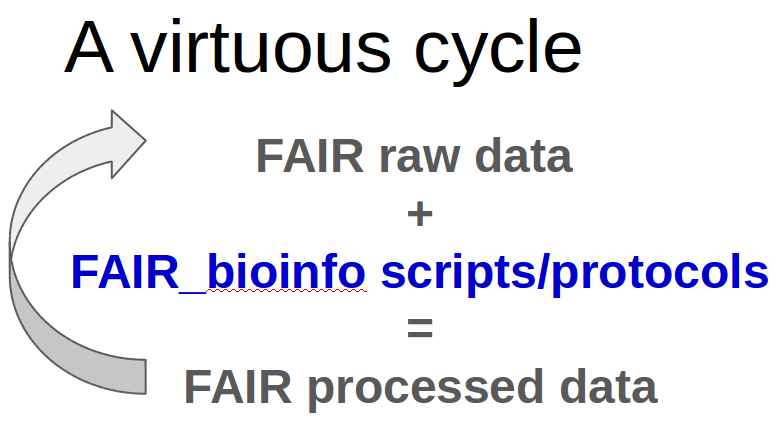
\includegraphics[height=3cm]{09_conclusion/images/FAIR_virtuousCircle.png}
\end{center}
\end{frame}
%-------------------------------------------
\begin{frame}{Swedish similar tutorial}
%\begin{columns}
%\begin{column}{0.6\textwidth}
\begin{center}
From the NBIS -- National Bioinformatics Infrastructure Sweden
    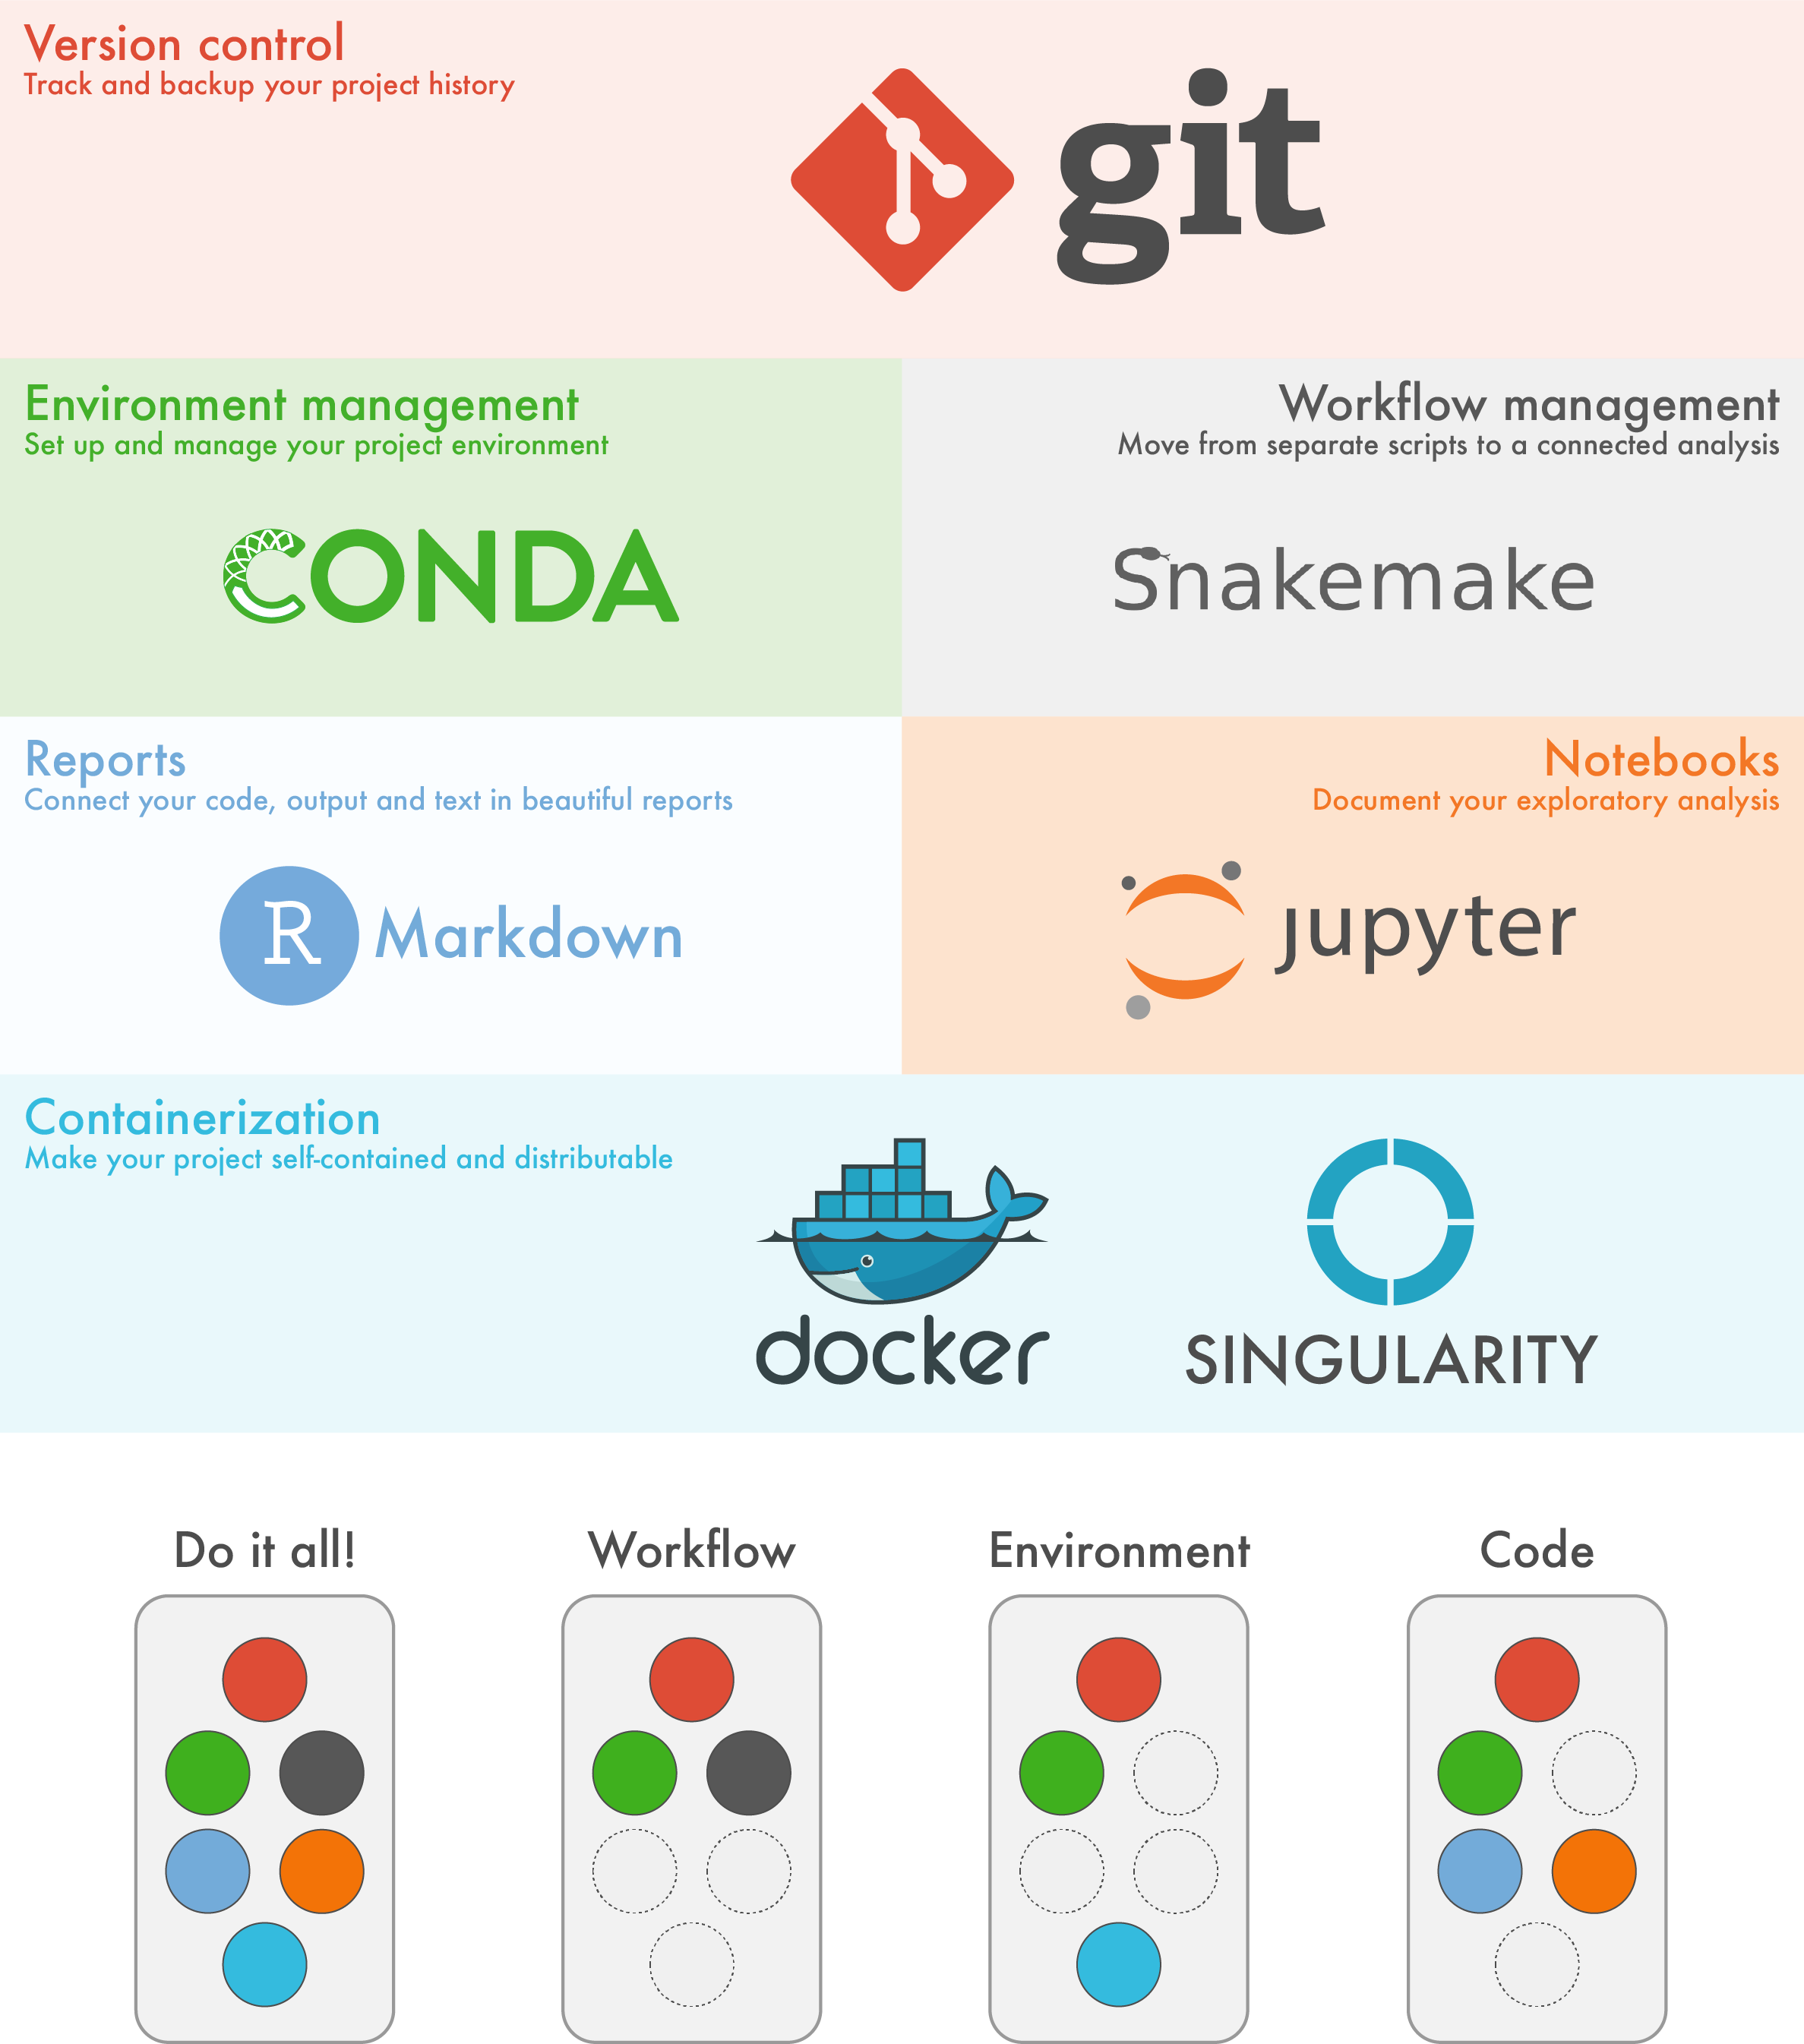
\includegraphics[width=6.3cm]{09_conclusion/images/NBIS_tutorials_overview.png}
%\end{center}
%\end{column}
%\begin{column}{0.3\textwidth}
%\begin{center}
    %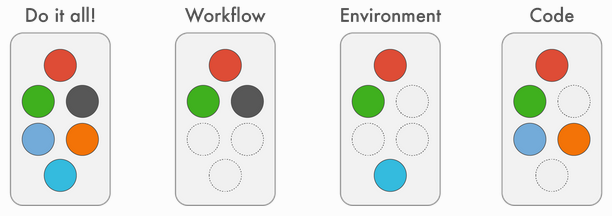
\includegraphics[width=6cm]{09_conclusion/images/NBIS_learning_scheme.png}
    \href{https://nbis-reproducible-research.readthedocs.io/en/latest/}{\textcolor{blue}{nbis-reproducible-research.readthedocs.io/en/latest}}
\end{center}
%\end{column}
%\end{columns}
\end{frame}
%---------------------------------------------------------
\begin{frame}{Reproducibility checklist\footnote{\href{https://www.nature.com/articles/d41586-020-02462-7}{\textcolor{blue}{\underline{Nature}}}}}

\begin{itemize}
    \item \textcolor{blue}{Code} \textcolor{violet}{avoid} workflows based on \textcolor{violet}{point-and-click interfaces} (eg. Excel), enshrine computations and data manipulation in code
    \item \textcolor{blue}{Document} how code works, define parameters and computational environment required: comments, \textcolor{violet}{notebooks} and README
    \item \textcolor{blue}{Record} key parameters (eg. the ‘seed’ values of a random-number generator)
    \item \textcolor{blue}{Test} functions using positive and negative control \textcolor{violet}{data sets}, run those tests throughout development
    \item \textcolor{blue}{Guide} with master script (eg. ‘run.sh’) that downloads data sets and executes workflow
    \item \textcolor{blue}{Archive} with long-term stability services such as Zenodo, Figshare and Software Heritage (GitHub is impermanent online repository)
\end{itemize}
\end{frame}

%---------------------------------------------------------
\begin{frame}{Reproducibility checklist\footnote{\href{https://www.nature.com/articles/d41586-020-02462-7}{\textcolor{blue}{\underline{Nature}}}}}

\begin{itemize}
    \item \textcolor{blue}{Track} the project’s history with a \textcolor{violet}{version-control} tools (eg. Git). Note (tag) which version you used to create each result
    \item \textcolor{blue}{Package} with ready-to-use computational environments using \textcolor{violet}{containerization} tools (eg. Docker, Singularity), web services (Code Ocean, Gigantum, Binder) or \textcolor{violet}{virtual-environment managers} (Conda)
    \item \textcolor{blue}{Simplify} and avoid niche or hard-to-install third-party code libraries
    \item \textcolor{blue}{Verify} your code’s portability by running it in a range of computing environments
    \item \textcolor{blue}{Automate} the test of your code with \textcolor{violet}{continuous-integration} services (eg. Travis CI)
\end{itemize}
\end{frame}    
%---------------------------------------------------------
\begin{frame}[containsverbatim]
\frametitle{Adding Tests}
\begin{block}{Unit test: test a part of the code}
\begin{columns}
\column{0.5\textwidth}
\begin{lstlisting}[language=python]
## module 1
sum <- function(x, y){
    return (x+y)
}

# Unit test
sum(2,2) == 4
\end{lstlisting}
\column{0.5\textwidth}
\begin{lstlisting}[language=python]
## module 2
power <- function(x, y){
    return (x**y)
}

# Unit test
power(2,2) == 4
\end{lstlisting}
\end{columns}
\end{block}
\begin{block}{Functional test: test all the code}
\begin{lstlisting}[language=python]
# Functional test
power(sum(2,2),2) == 16
\end{lstlisting}
\end{block}
\end{frame}

%---------------------------------------------------------
\begin{frame}{Continuous integration}

Automated verification each time the source code is modified that the modifications do not produce:
\begin{itemize}
    \item any regression in the developed application
    \item any change in the results obtained
\end{itemize}
\begin{columns}
\column{0.30\textwidth}
\begin{center}
    \href{https://docs.travis-ci.com/user/tutorial/}{
\includegraphics[height=1.5cm]{09_conclusion/images/FAIR_travisCI_logo.png}}
    \href{https://circleci.com/integrations/github/}{
\includegraphics[height=2cm]{09_conclusion/images/FAIR_CircleCI_logo.png}}
\end{center}
\column{0.65\textwidth}
\begin{center}
    \href{https://circleci.com/integrations/github/}{
\includegraphics[height=3cm]{09_conclusion/images/FAIR_Github_Actions.png}}
    \end{center}
\end{columns}
 \end{frame}
%-------------------------------------------
\begin{frame}{Reproducibility: a multidimensional and multi-level process}

\begin{center}
    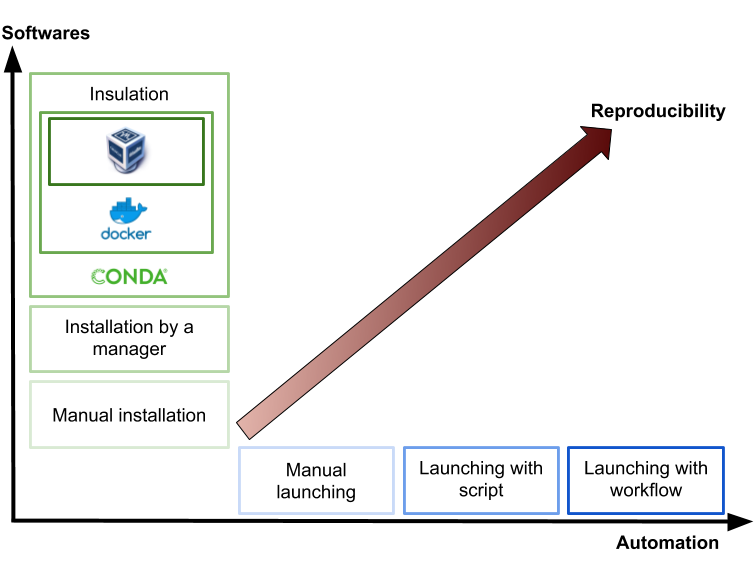
\includegraphics[width=10cm]{09_conclusion/images/FAIR_2d_reproducibility.png}
\end{center}

\end{frame}
%---------------------------------------------------------
%\begin{frame}{What now?}
%
%A few propositions to go further... \newline
%
%See: Practical Computational Reproducibility in the Life Sciences, Björn Grüning et al, 2018\par
%
%\begin{itemize}
%    \item Install your software using Conda or Docker
%    \item Create virtual machines / images and share them
%    \item Continuous integration
%\end{itemize}
%
%\end{frame}

%---------------------------------------------------------
\begin{frame}{\FAIRB}

\begin{columns}
\begin{column}{.55\textwidth}
\begin{block}{Automation}
\begin{center}
    Manual command lines\\
    $\downarrow$\\
    Write a shell script\\
    $\downarrow$\\
    Use a workflow manager\\
    $\downarrow$\\
    Tests and continuous integration (*)
\end{center}
\end{block}
\begin{block}{User analysis (trial-and-error)}
\begin{center}
    Offer a GUI (eg. with R-Shiny) (*)\\
    $\downarrow$\\
    Save and re-import choices (*)
\end{center}
\end{block}
\end{column}
\begin{column}{.35\textwidth}
\begin{block}{Softwares}
\begin{center}
Local installation\\
$\downarrow$\\
Package manager\\
$\downarrow$\\
Conda environment\\
$\downarrow$\\
Image / container\\
$\downarrow$\\
Virtual machine (*)
\end{center}
\end{block}
\end{column}
\end{columns}
\begin{center}
    (*) not carried out in the course
\end{center}
\end{frame}
%-------------------------------------------
\begin{frame}{\FAIRB}

\begin{center}
    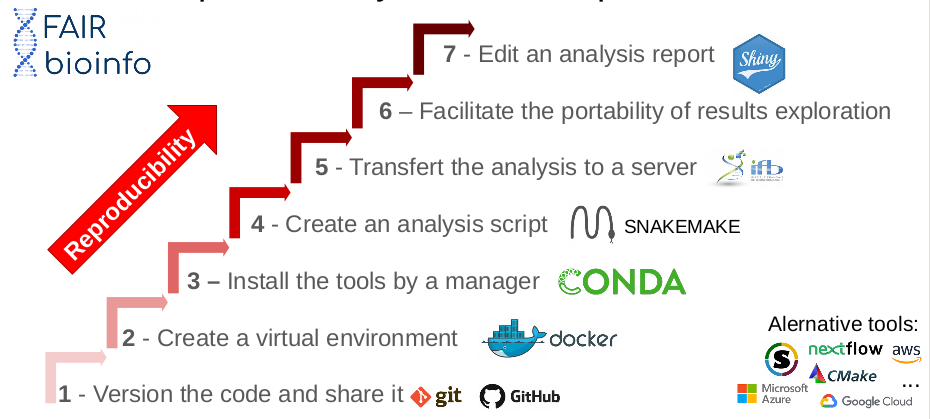
\includegraphics[width=12cm]{09_conclusion/images/FAIR_7steps_reproducibility.png}
\end{center}

\end{frame}

%---------------------------------------------------------
%\begin{frame}{}
%\huge{So... What now?}
%\end{frame}

 %---------------------------------------------------------
\begin{frame}{Reproducibility - how far?}
\begin{columns}
\column{0.55\textwidth}
\begin{block}{Reproducibility to the exact bit?}

\includegraphics[height=0.3cm]{05_history/Images/FAIR_no.png} container uses some resources of the support machine\\

\includegraphics[height=0.3cm]{05_history/Images/FAIR_yes.png} version control of the env. (Nix, Guix)
\end{block}
\column{0.42\textwidth}
%\begin{block}{FAIR$\_$bioinfo training}
%
\includegraphics[height=0.3cm]{05_history/Images/FAIR_no.png} use of an already instantiated VM\\
%
\includegraphics[height=0.3cm]{05_history/Images/FAIR_yes.png} create your own VM image
%\end{block}

\begin{block}{HPC and parallelization?}
 
\includegraphics[height=0.3cm]{05_history/Images/FAIR_no.png} loss of computanional order, multi-threading, identical hardware?\\
 
\includegraphics[height=0.3cm]{05_history/Images/FAIR_yes.png} ...?
\end{block}
\end{columns}
\begin{center}
    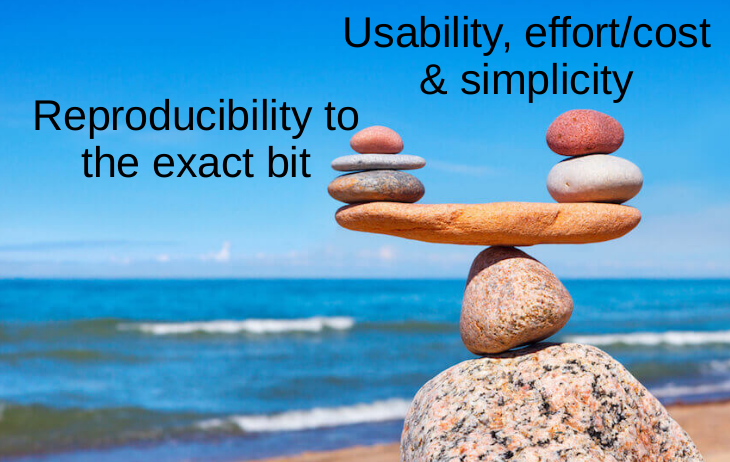
\includegraphics[height=4.8cm]{shared/FAIR_equilibre.png}
\end{center}
\end{frame}
%-----------------------------------------------------
\begin{frame}{Thanks}
\begin{itemize}
    \item Organizational comity (our guardian angels): Yousra, Hélène
    \item IFB Core Cluster taskforce: Julien, Gildas, and all those who provide in the shadows
    \item Helpers: Paulette, Emilie, Pauline, Hugo
    \item Organisations: CNRS, INRAE, IFB, I2BC, Paris Saclay University
\end{itemize}
\end{frame}
